\section{CMB Maps from Generalised Local NonGaussianity}
\begin{itemize}
\item Description of the form of nonGaussianity produced by these models.
\item Description of how to do marginalisation from coarse-grained distribution (ie. smoothed over a Hubble at the end of inflation) to pixels in CMB of LSS
\item T and E maps from generalised local nonGaussianity
\end{itemize}

For an observer,  the primordial comoving curvature fluctuations  $\zeta$ can be expanded with spherical harmonics
\begin{equation}
  \zeta(r, \mathbf{n}) = \sum_{lm} Y_{lm}(\mathbf{n})\zeta_{lm}(r),
\end{equation}
where $r$ is the distance from the observer and $\mathbf{n} = (\theta, \phi)$ the line of sight direction. For linear projection, the projected temperature harmonic coefficient $a_{lm}^T$ is a superposition of $\zeta_{lm}(r)$ with appropriate weights $F_l^T(r)$. In this subsection we derive $F_l^T(r)$ and describe the numeric techniques to compute it.

 For a comoving wave number $\mathbf{k}$, the Fourier mode $\zeta_{\mathbf{k}}$ can be written as
\begin{equation}
  \zeta_{\mathbf{k}} = 4\pi \int_0^\infty r^2dr\sum_{lm}\zeta_{lm}(r) (-i)^l j_l(kr) Y_{lm}(\hat{\mathbf{k}})\, , \label{eq:zetakint}
\end{equation}
where we have used the identity
\begin{equation}
  e^{i\mathbf{k}\cdot\mathbf{n}r} = 4\pi \sum_{lm}i^l j_l(kr) Y^*_{lm}(\hat{\mathbf{k}}) Y_{lm}(\mathbf{n}) \, , \label{eq:eikx_expand}
\end{equation}
and orthogonality of $Y_{lm}$ functions.


The temperature field can be integrated along the line of sight
\begin{equation}
T({\mathbf{n}}) = \int S_T(\mathbf{k}, r') e^{i \mathbf{k}\cdot\mathbf{n} r'}\zeta_{\mathbf{k}}\frac{d^3k}{(2\pi)^3}, \label{eq:Tint1}
\end{equation}
where $S(\mathbf{k}, r')$ is the source function that can be computed using a Boltzmann code.

Plugging \eqref{eq:zetakint} and \eqref{eq:eikx_expand} into \eqref{eq:Tint1}, we obtain the desired expression
\begin{equation}
a_{lm}^T = \int_0^\infty \zeta_{lm}(r) F^T_l(r) dr, \label{eq:Tint2}
\end{equation}
where
\begin{equation}
F^T_l(r) = \frac{2r^2}{\pi} \int k^2dk j_l(kr) \int dr' S_T(k, r') j_l(kr') \, . \label{eq:FTint}
\end{equation}

Although it seems to be profitable to convert the 3D integral problem to a 2D integral problem by first integrating over $r'$ in \eqref{eq:FTint} and saving the $r$-indepedent result for all $r$ values in eq.~\eqref{eq:Tint2}, practically it is not the case. The problem can be explictly seen from the identity
\begin{equation}
\int_0^\infty k^2 j_l(kr) j_l(kr') = \frac{\pi}{2r^2}\delta(r - r') \,. \label{eq:jljlint}
\end{equation}
If $S(k, r')$ is $k$-independent and we integrate over $r'$ first, we will be computing a Dirac delta function numerically. To avoid that, we split r.h.s. of eq.~\eqref{eq:FTint} into an instant-recombination term and a correction term:
\begin{equation}
F^T_l(r) =  S\left(\frac{l+1/2}{r}, r\right) + \frac{2r^2}{\pi} \int k^2dk j_l(kr) \int dr' \left[S(k, r')- S\left(\frac{l+1/2}{r'}, r'\right)\right] j_l(kr') \, , \label{eq:FTint2}
\end{equation}
where eq.~\eqref{eq:jljlint} has been used.

The removal of an implicit Dirac delta function improves the numeric stability. However, we are still facing the problem that the amplitude of $k^2 j_l(kr) j_l(kr')$ diverges at high $k$. Fortunately the source $S(k, r')$ is relatively smooth along $k$ direction. It acts as a low-pass filter on $k^2j_l(kr)j_l(kr')$. The numeric accuracy can be greately improved by doing a WKB expansion of $k^2j_l(kr)j_l(kr')$ and keeping only the low frequency part of it. The high frequency part of $k^2j_l(kr)j_l(kr')$ adds fast-oscillating cosine noises, which have negligible contribution to the total integral. The robustness of this method can be tested by varying the frequency cutoff for the low-pass filtering and observe the stability of the result.

The $\chi$ to $\zeta$ mapping is defined for a given scale $L$. The $L^3$-volume averaged $\bar{\zeta}|_{L^3}$ is a function of the averaged $\bar{\chi}|_{L^3}$.
\begin{equation}
\bar{\zeta}\vert_{L^3}  = f\left(\bar{\chi}\vert_{L^3}\right)\, .
\end{equation}

The random Gaussian $\chi$ field can be realized in discrtized shells with known covariance matrix:
\begin{eqnarray}
  \langle \chi^*_{lm}(r) \chi_{l'm'}(r')\rangle &=& \frac{\pi^2}{2^{2-n_s}}  \delta_{ll'}\delta_{mm'} \mathcal{P}_S\left(\frac{2}{r+r'}\right) \left(\frac{2\max(r,r')}{r+r'}\right)^{1-n_s} \left(\frac{\min(r, r')}{\max(r,r')}\right)^l \label{eq:chilmcov} \\
 &&  \times \frac{\Gamma\left(l+\frac{n_s-1}{2}\right)}{\Gamma\left(l+\frac{3}{2}\right)\Gamma\left(4-n_s\right)} {\ _2F_1\,}\left( \frac{n_s}{2}-1,\, l+\frac{n_s-1}{2},\, l+ \frac{3}{2},\, \left(\frac{\min(r, r')}{\max(r,r')}\right)^2\right)     \nonumber \, , 
\end{eqnarray}
where $\mathcal{P}_S\equiv \propto k^{n_s-1} $ is the power spectrum of $\chi$. The function $\,_2F_1$ is the ordinary hypergeometric function and $\Gamma$ the Gamma function.


\begin{figure}
  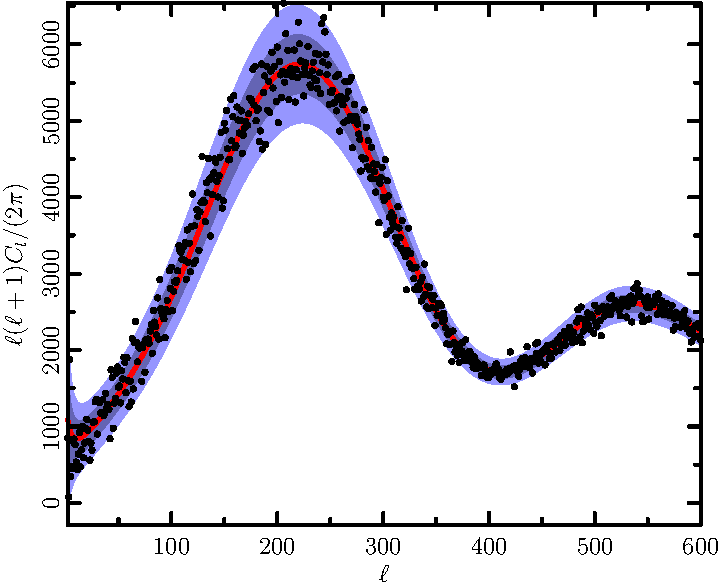
\includegraphics[width=\textwidth]{ClTT_proj.pdf}
  \caption{The black dots are projected $C_\ell^{TT}$ for $\Lambda$CDM model, where $\zeta_{lm}(r)$ are realized using the covariance matrix in eq.~\eqref(eq:chilmcov} ($\chi$ replaced with $\zeta$) and $a_{lm}$ are computed using eq.~\eqref{eq:Tint2}. The solid red line is the theoretical ensemble average of $C_\ell^{TT}$. The dark and light blue regions are $1\sigma$ and $2\sigma$ limits of cosmic variance.}
\end{figure} 


At high resolution ($\ell \gtrsim 1000$) CMB lensing starts to kick in and linear transfer is not sufficiently accurate. We restrict the discussion in this paper to angular scales $\ell \lesssim 1000$ and leave the sophistication beyond linear transfer to our future work.


